\documentclass{article}

\usepackage[margin=1in]{geometry}
\usepackage{graphicx}
\usepackage{amsmath}

\setlength{\parindent}{0pt}

\begin{document}

\noindent 18-748 Lab 1 \hfill Group 17

\noindent \hrulefill

\section*{Assignment 2}

\begin{center}
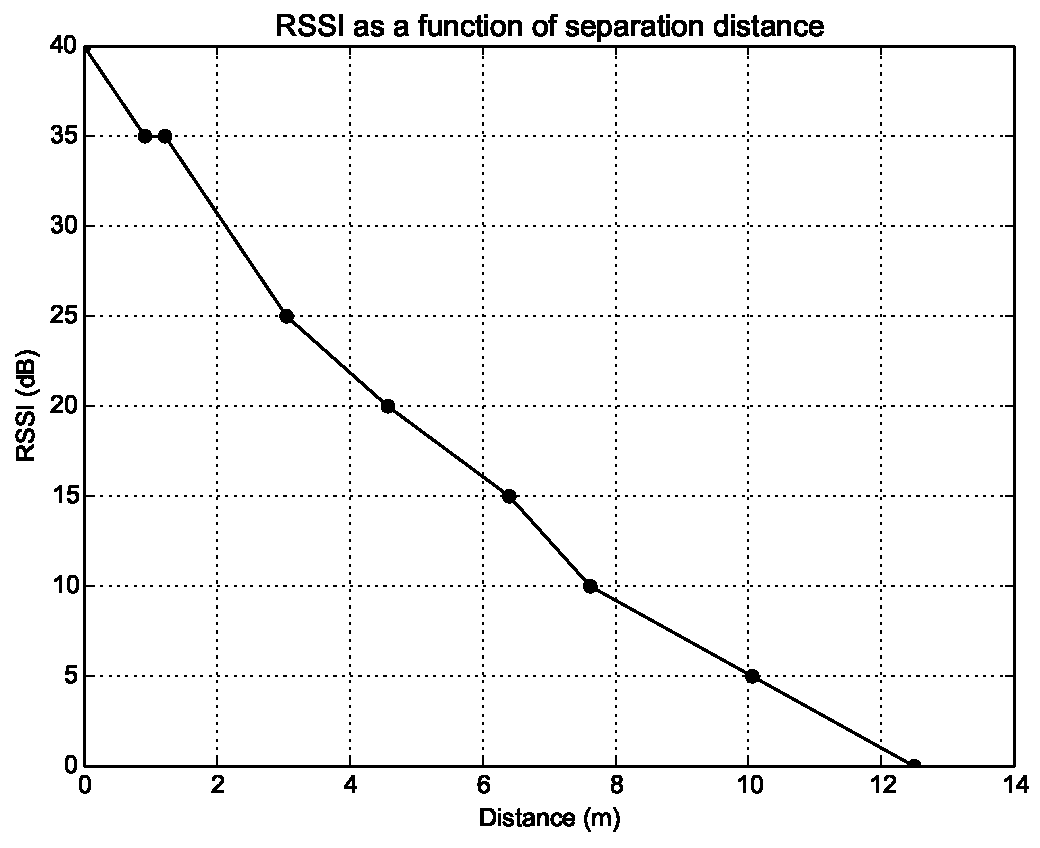
\includegraphics[width=4in]{rssi-vs-dist}
\end{center}

Path loss is defined as a function of distance $d$
\[
    L = 10 n \log_{10} d + C
\]
where $n$ is the unknown path loss exponent and $C$ is an unknown constant.

Path loss is an additive inverse of RSSI (the weaker the signal, the higher the
loss):
\[
    L = -\text{RSSI}
\]

Each measured data point ($d_i, \text{RSSI}_i)$ provides one equation that
determines $n$ and $C$:
\[
    \text{RSSI}_i = 10 n \log_{10} d_i + C
\]
The set of all data points together form an over-determined system of linear
equations.

To calculate the path loss exponent we solve the above over-determined linear
system of equations by finding the least-squares solution, i.e. the solution
$(n, C)$ that minimizes the sum of squares of the residuals:
\[
\sum_i (10 n \log_{10} d_i + C - \text{RSSI}_i)^2
\]

The code that does this is in \texttt{path-loss-exp.py}.

% $ ./path-loss-exp.py -s 6 4 -f path-loss-lstsq.eps rssi-vs-dist.conv.csv 
% n = 2.51243133312 C = -33.0140444725
The least-squares solution for our data points is $n = 2.51$ and $C = -33.01$.
The residuals are shown on the following figure as the vertical distances
between the points and the curve.

\begin{center}
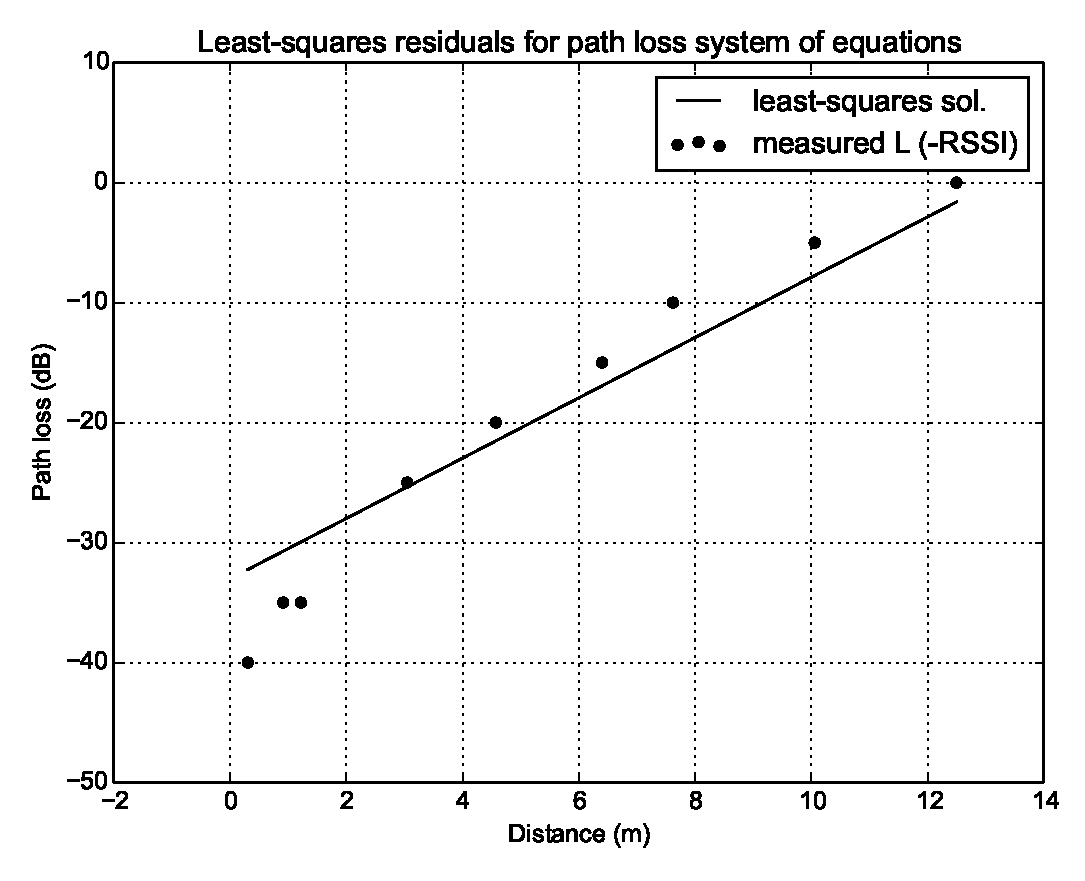
\includegraphics[width=4in]{path-loss-lstsq}
\end{center}

\section*{Assignment 3}

Job response time statistics computed by code given in \texttt{response-time.py}:

Priority(Task 1) = 1 \\
Priority(Task 2) = 2

\begin{verbatim}
            response_s
task
1    count   21.000000
     mean     0.441406
     std      0.151471
     min      0.281250
     25%      0.291016
     50%      0.441406
     75%      0.591797
     max      0.601563
2    count   11.000000
     mean     0.277166
     std      0.046275
     min      0.138672
     25%      0.285156
     50%      0.290039
     75%      0.294922
     max      0.299805
\end{verbatim}

Priority(Task 1) = 2 \\
Priority(Task 2) = 1

\begin{verbatim}
            response_s
task
1    count   31.000000
     mean     0.278793
     std      0.033786
     min      0.102539
     25%      0.276855
     50%      0.284180
     75%      0.291504
     max      0.298828
2    count   16.000000
     mean     0.576538
     std      0.046188
     min      0.406250
     25%      0.579590
     50%      0.586914
     75%      0.594238
     max      0.601563
\end{verbatim}

From the statistics we see that in the first scenario response time of Task 1
ranges from 300 ms to 600ms (about half of each). This is because Task 1 is
preempted by Task 2 when both are ready at the same time (which happens half
the time). In the second scenario, Task 1 is highest priority, so it always
completes within 300 ms regardless of what Task 2 is doing. Task 2 has to wait
for Task 1, which increases its maximum response time to 600 ms.

\subsection*{Bonus 1: tight CPU reserve}

When a task has highest priority it receives no interference from other tasks,
and its response time in that case equals its execution time (ignoring
overhead).  From statistics from first scenario above (Task 2 highest
priority), we see that Task 2 max response time is 299 ms ($<= 300$ ms). From
second scenario (Task 1 highest priority), we see that Task 1 response time is 
298 ms ($<= 300$ ms).

However, our measurement of completion time is an underestimate, because it
does not include the printf() call as well as some small overhead of the
``first half'' of the \texttt{wait\_for\_next\_period} call. As a result, we
need to expand our measured budget of 300 ms. An additional 5 ms does the
trick. With budgets of 305 ms the tasks work correctly.

\pagebreak

\subsection*{Bonus 2: execution state plot}

Context switch event collected by a \texttt{printf} statement added to
\texttt{\_nrk\_scheduler} and configuring \verb!NRK_NO_POWER_DOWN!  because
otherwise the print output is half-broken upon context switches into the idle
task. Python scripts for parsing trace and drawing plot in \texttt{assignment3}
directory.

\vspace{10pt}

Priority(Task 1) = 1 \\
Priority(Task 2) = 2
\begin{center}
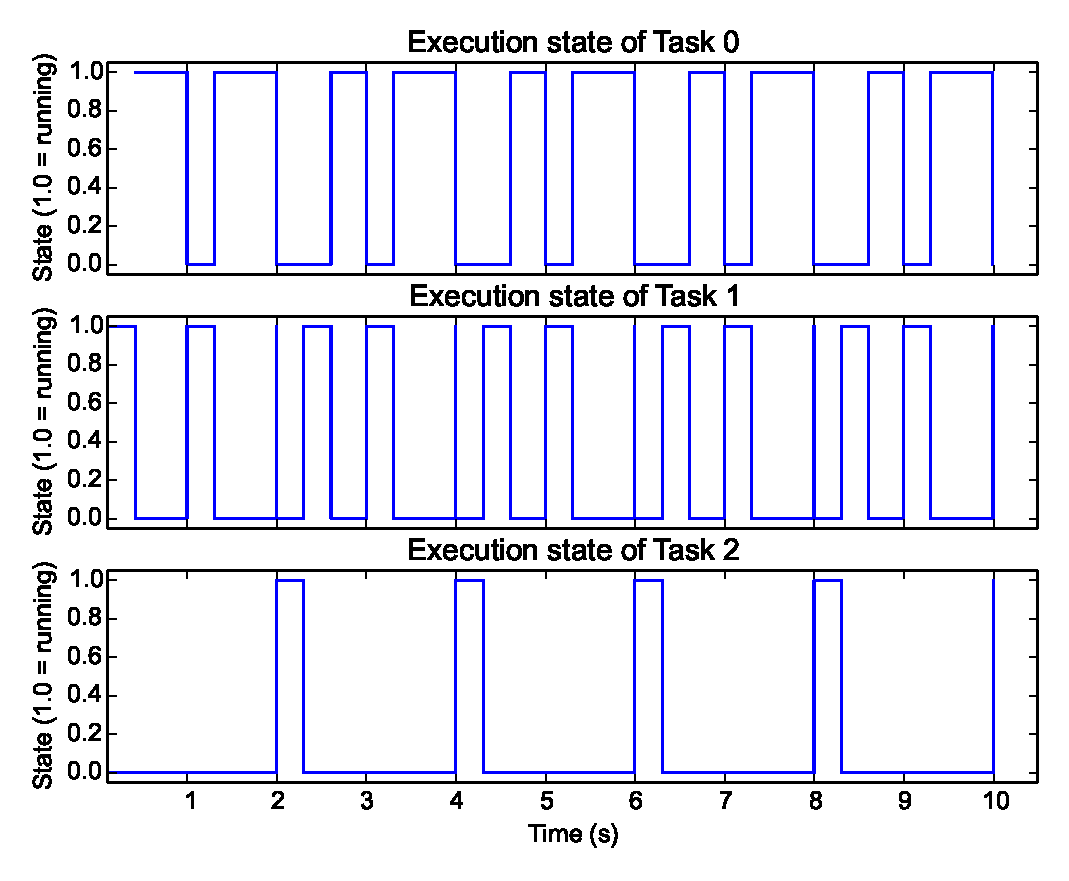
\includegraphics[width=4in]{ctx-switch-trace-orig}
\end{center}

Priority(Task 1) = 2 \\
Priority(Task 2) = 1
\begin{center}
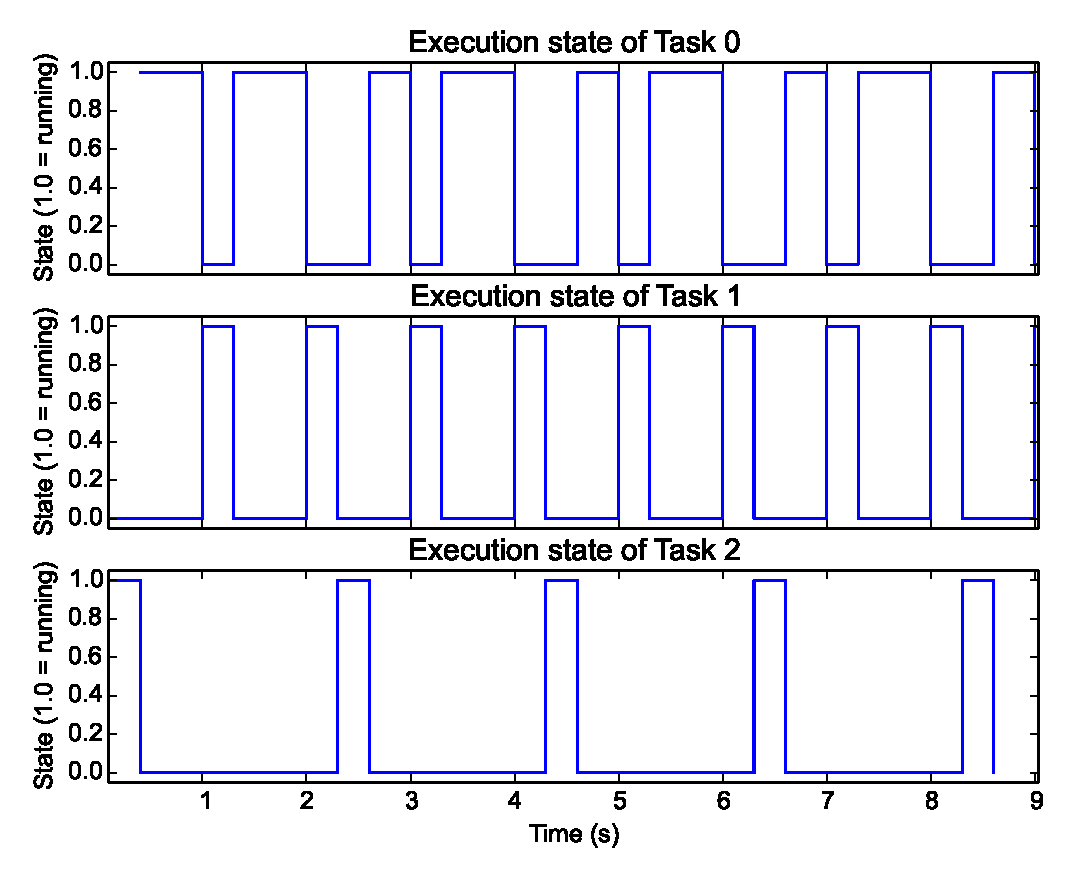
\includegraphics[width=4in]{ctx-switch-trace-flipped}
\end{center}

\end{document}
